\chapter{Experimental Setting}
This section provides a broad overview of foundational ideas
and background material relevant to this thesis.
In most chapters of this thesis, we include a deeper
discussion of the related literature relevant to
that material.


\section{Experimental Setting}
\subsection{Self-supervised Exploration}
% explain why this setting is important, and explain the baselines 
We assume that we have an unlabeled target dataset of images for which we would like to learn useful visual features. We compare three methods:
% EB: we should consider a better abbreviated method name. how about: IE, IE+?
% \begin{enumerate}[noitemsep,topsep=0pt]
%     \item Random: sample queries uniformly at random from the vocabulary. 
%     \item Ours: sample queries from our learned concept distribution. 
%     \item Ours++: additionally use GPT-generated descriptors
% \end{enumerate}
\begin{enumerate}[noitemsep,topsep=0pt]
    \item Random: sample concepts uniformly from the vocab. 
    \item Ours: sample concepts from our learned distribution. 
    \item Ours++: additionally use GPT-generated descriptors.
\end{enumerate}

\begin{figure*}[t]
    \centering
    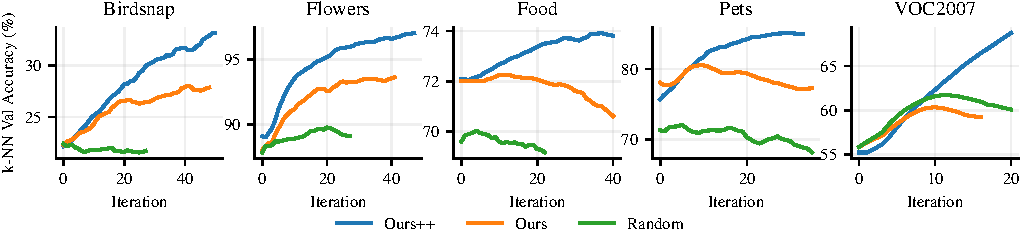
\includegraphics[width=\linewidth]{figures/ssl-curves-updated.pdf}
    \vspace{-2.4em}
    \caption{\textbf{Learning curves in self-supervised setting.} We show how $k$-NN validation accuracy improves across iterations on each target dataset. Without using any labels, Internet Explorer identifies and focuses on relevant concepts for each target dataset. This allows it to find more useful data than the baseline that searches for random concepts. Adding GPT-generated descriptors (Ours++) further improves performance by enabling Internet Explorer to generate diverse views of useful concepts. 
    % Interestingly, the random baseline does quite well on VOC2007, perhaps because coarse-grained classification benefits from a broader variety of training data. 
    } 
    \label{fig:learning_curves}
\end{figure*}

\subsection{Label Set-guided Exploration}
% explain why this setting is also potentially practical 
% explain the baselines 
We may sometimes know the set of labels for our task (e.g., ``golden retriever'', etc.) even if we do not have image-label pairs. 
Knowing the label set greatly accelerates learning on the Internet, because it acts as a strong prior on what could be useful. 
Using our text similarity model, we reduce the size of the vocabulary by selecting the top 
% 10,000 concepts
$10\%$ ($14{,}635$ concepts)
with the largest average top-$k$ similarity to the label set in text embedding space. We set $k$ to a third of the size of the label set to reduce the impact of outliers. Reducing the size of the vocabulary strengthens our baselines by ensuring that they only search for potentially useful concepts. We compare 4 methods:   
\begin{enumerate}[noitemsep,topsep=0pt]
    \item Labels: only search for labels. 
    \item Labels + relevant: search for labels \todo{is it worth making ``half'' a param?} half of the time, and random concepts from the pruned vocabulary the other half of the time. 
    \item Ours: sample labels half of the time and sample from our learned concept distribution the other half. 
    \item Ours++: additionally use GPT-generated descriptors.
\end{enumerate}
% We call this setting ``semi-supervised,'' since we have additional supervision in the form of the label set.
We call this setting ``label set-guided,'' since we have additional supervision in the form of the label set.
% Note that this is different from the typical semi-supervised learning setting, which learns from a fixed labeled dataset and a fixed unlabeled dataset.
% Note that this differs from the typical semi-supervised learning setting, which learns from fixed labeled and unlabeled datasets.

\subsection{Datasets and Metrics}
We evaluate Internet Explorer on 4 popular small-scale fine-grained classification datasets: Birdsnap~\cite{berg2014birdsnap}, Flowers-102~\cite{nilsback2008automated}, Food101~\cite{bossard2014food}, and Oxford-IIT Pets~\cite{parkhi2012cats}.
% which are commonly used to evaluate transfer learning for large pre-trained models~\cite{kornblith2019better}. 
We also evaluate on Pascal VOC 2007 (Cls)~\cite{everingham2010pascal}, a coarse-grained multi-label classification task. Finally, we try fMoW~\cite{fmow2018}, a satellite domain classification task. These small datasets consist of $2{,}040$ to $75{,}750$ training examples, making them ideal for testing whether Internet Explorer can efficiently find relevant useful data.
\todo{hammer home that we are using a \textit{single} dataset not doing general purpose here?}
We do not target large-scale datasets like ImageNet~\cite{deng2009imagenet} because they already contain over a million human-curated Internet images.
We compare the representation quality of our model \wrt~its target dataset using two metrics: $k$-nearest neighbors ($k$-NN) accuracy and linear probe accuracy. 
% $k$-NN accuracy can be computed quickly, so we use this to plot learning curves of model performance after every iteration during training. We report the early-stopped linear probe accuracy in our tables.

% \subsection{Evaluation Metrics}
% We compare the representation quality of our models using two metrics: k-nearest neighbors (k-NN) accuracy  and linear probe accuracy. To measure k-NN accuracy, we use our ResNet-50 to encode each dataset's training and test sets. Then, for each test example, we find its $k$ nearest neighbors in representation space and use the mode of its neighbors' labels as the prediction. We use k-NN accuracy to plot learning curves of model performance after every iteration, since it is easy to quickly compute. 
% To compute the linear probe accuracy, we again use our Resnet-50 model to encode each dataset's training and test sets. Then we learn a linear head on top of fixed training representations by minimizing the cross-entropy loss. We tune the weight decay parameter in the range $(10^{-6}, 10^6)$, as is done in~\cite{radford2021learning}.


% \subsection{Metrics}
% We evaluate compare models using the k-nearest neighbors accuracy to compare their representation qualities. For each validation image, we determine its nearest neighbors in the training set using the cosine similarity of their representations. We select $k$ by maximizing the validation accuracy. In contrast to other metrics like fine-tuning or linear probe accuracy, k-NN accuracy is fast and easy to compute. Beyond accuracy, we also prefer models that were trained using fewer GPUs, in less time, using as few images as possible.  


\begin{table*}[t]
    \centering
    \begin{adjustbox}{width=1\textwidth}
    \begin{tabular}{lc@{\hskip 0.12em}cc@{\hskip 0.12em}cc@{\hskip 0.12em}cc@{\hskip 0.12em}cc@{\hskip 0.12em}cc@{\hskip 0.12em}cc@{\hskip 0.12em}cc}
    \toprule
        % Model & Flowers102 & Food101 & Stanford Cars & Oxford-IIIT Pets & Total Images & GPU-hours \\
        Model & \multicolumn{2}{l}{Birdsnap} & \multicolumn{2}{l}{Flowers} & \multicolumn{2}{l}{Food}  & \multicolumn{2}{l}{Pets} & \multicolumn{2}{l}{VOC2007} & \multicolumn{2}{l}{fMoW} & Images & GPU-hours \\
    \midrule
    \textit{Fixed dataset, language supervision} \\
        \;\;\;CLIP ResNet-50 (\textbf{oracle \& 2x params})  & $57.1$ & & $96.0$ & & $\bf{86.4}$ & & $88.4$ & & $\bf{86.7}$ & & 37.5 & & $400 \times 10^6$ & $4{,}000$ \\ % 82.8 for CLIP pascal 
    \midrule
    \textit{Fixed dataset, self-supervised} \\
        \;\;\;MoCo-v3 (ImageNet pre-train)  & $26.8$ & & $83.2$ & & $70.5$ & & $79.6$ & & $-$ & & 32.6 & &  $1.2 \times 10^6$ & $72$ \\
        %\;\;\; MoCo-v3 (target only)                      & 80.0 & 0    & 0    & $< 10^5$ & 2 \\
        \;\;\;MoCo-v3 (ImageNet + target)  & $39.9$ & & $94.6$ & & $78.3$ & & $85.3$ & & $58.0^\dag$ & & 48.8 & & $1.2 \times 10^6$ & $72 + 12$ \\
    \midrule
    \textit{No label set information} \\
        \;\;\;Random exploration  & $39.6$ & \red{$(-0.3)$} & $95.3$ & \green{$(+0.7)$} & $77.0$ & \red{$(-1.3)$} &  $85.6$ & \green{$(+0.3)$} & $70.2$ & \green{$(+12.2)$} & $-$ & &  $2.2 \times 10^6$ & $84 + 40$ \\
        \;\;\;Ours  & $43.4$ & \green{$(+3.5)$} & $97.1$ & \green{$(+2.5)$} & $80.5$ & \green{$(+2.2)$} & $86.8$ & \green{$(+1.5)$} & $68.5$ & \green{$(+10.5)$}  & $-$ & & $2.2 \times 10^6$ & $84 + 40$ \\
        \;\;\;Ours++  & $54.4$ & \green{$(+14.5)$} & $98.4$ & \green{$(+3.8)$} & $82.2$ & \green{$(+3.9)$} & $89.6$ & \green{$(+4.3)$} & ${80.1}$ & \green{${(+22.1)}$} & $-$ & & $2.2 \times 10^6$ & $84 + 40$ \\
    \midrule 
    \textit{Use label set information} \\       
        \;\;\;Search labels only  & $47.1$ & \green{$(+7.2)$} & $96.3$ & \green{$(+1.7)$} & $80.9$ & \green{$(+2.6)$} & $85.7$ & \green{$(+0.4)$} & $61.8$ & \green{$(+3.8)$} & $49.3$ &  \green{$(+0.5)$} & $2.2 \times 10^6$ & $84 + 40$ \\
        \;\;\;Labels + relevant terms  & $49.9$ & \green{$(+10.0)$}& $98.0$ & \green{$(+3.4)$} & $81.2$ & \green{$(+2.9)$} & $87.0$ & \green{$(+1.7)$} & $67.5$ & \green{$(+9.5)$} & $-$ & & $2.2 \times 10^6$ & $84 + 40$ \\
        \;\;\;Ours  & $52.0$ & \green{$(+12.1)$} & $97.6$ & \green{$(+3.0)$} & $81.2$ & \green{$(+2.9)$} & $87.3$ & \green{$(+2.0)$} & $70.3$ & \green{$(+14.3)$} & $-$ & & $2.2 \times 10^6$ & $84 + 40$ \\
        \;\;\;Ours++  & $\mathbf{62.8}$ & \green{$\mathbf{(+22.9)}$} & $\bf{99.1}$ & \green{$\mathbf{(+4.5)}$} & $84.6$ & \green{$(+6.3)$} & $\mathbf{90.8}$ & \green{$\mathbf{(+5.5)}$} & ${79.6}$ & \green{$(+21.6)$} & $\bf{50.6}$ & \green{$\mathbf{(+1.8)}$} & $2.2 \times 10^6$ & $84 + 40$ \\
    \bottomrule
    \end{tabular}
    \end{adjustbox}
    \vspace{-0.1in}
    % \caption{\textbf{Linear probe accuracy on targeted datasets}.}
    \caption{\textbf{Linear probing accuracy}. Our method significantly improves the starting checkpoint performance in just 40 additional hours of training. We show the performance change from the starting MoCo-v3 (ImageNet + target) initialization in \green{green}/\red{red}. CLIP numbers correspond to linear probe (which is higher than its zero-shot accuracy). Internet Explorer reaches or often surpasses CLIP (oracle with 2x params) performance on each dataset while using 2.5\% as much compute and 0.5\% as much data. ${}^{\dag}$For VOC2007, we do not do ImageNet pre-training because ImageNet is too close to VOC2007.
    % obscures the effect of Internet Explorer. 
    % We report $k$-NN accuracy in the VOC2007 column and show LP in the supplementary. 
    }
    \label{tab:main_results}
    \vspace{-0.06in}
\end{table*}


\begin{figure}[t]
\centering
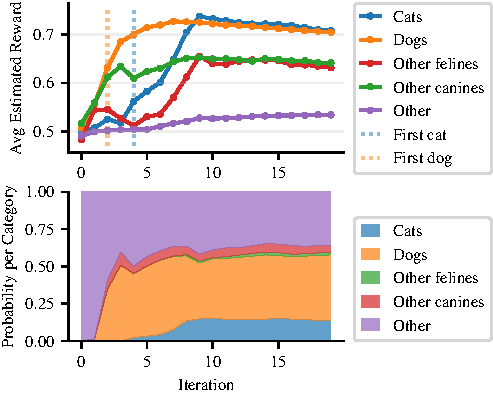
\includegraphics[width=0.8\linewidth]{figures/pets_ssl_reward_over_training2.pdf}
% 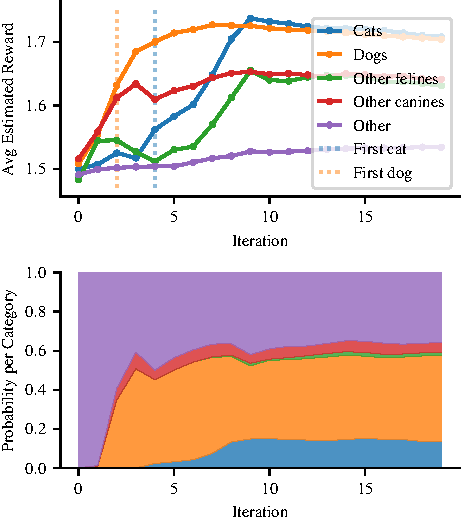
\includegraphics[width=0.82\linewidth]{figures/pets_ssl_reward_over_training.pdf}
\caption{\textbf{Self-supervised concept discovery on Pets dataset.} When targeting the Pets dataset, self-supervised Internet Explorer quickly estimates high reward for concepts from the cat category (82 concepts) and dog category (246 concepts). It is also able to identify felines that are not cats (e.g., tiger) and canines that are not dogs (e.g., wolf), although it gives them lower reward on average. Finding these categories is especially challenging, since they comprise only $460/146{,}347 = 0.3\%$ of the vocabulary.}
% \vspace{-0.17in}
\label{fig:reward_over_training}
\end{figure}


%%% Local Variables:
%%% coding: utf-8
%%% mode: latex
%%% TeX-engine: xetex
%%% TeX-master: "../thesis"
%%% End:
